\section{Methodology}
\label{sec:methodology}

\subsection{Data Preprocessing}
\label{subsec:preprocessing}
The first step is to acquire the data. Using the \textit{Yahoo Finance} tool for python, the data is easily fetched with using the company stock symbol and the historical period. After
it, an object containing the stock prices and some other informations will be acquired. In order to avoid fetching the same data every time the code in run and to avoid store everything 
on the RAM memory, there was developed a database to organize and store the data. This way, only new data will be fetched and stored. This database is designed to store data for any number
of companies.\\
\\
The database was organized in three tables:
\begin{itemize}
 \item \textbf{Companies:} Stores the Symbol and the Name of all listed companies.\\
 \item \textbf{Period:} Stores the period of the data stored of each company.\\
 \item \textbf{Data:} Store all the useful data of all companies.\\
\end{itemize}
\ \\
The Figure \ref{fig:db} shows the organization of the database.
\\
\begin{figure}[H]
\centering
\includegraphics[width=0.6\textwidth]{figures/database.png}
\caption{Organization of the tables.}
\label{fig:db}
\end{figure}
\ \\
With this process, the data need to be achieved before the processing. However, while the data from one company is being downloaded into the database, the next algorithm can be performed
to the data of a storage company. Also, the data of all wished companies can be downloaded into the database before starting. The positive point about this, is that RAM memory is saved
by storing data in hard disk. However, this database can grow as the hard disk supports, therefore it is important to not try to download all the data from every company in the stock market.
Once the data is organized in the database, the Preprocessing starts.\\
\\
In order to deal with the outliers points, the solution used was to implement the \textit{Savitzky–Golay filter}, which is a digital filter used to smooth the data\cite{filter}. This solution is 
easy to implement and works fine with this dataset, however, the challenge is to define the best parameters. It is common to conclude that the best parameters would be the ones that result in the 
best $R² score$. But, this would not smooth the curve, just fit it perfectly. Therefore, the best parameters should be the ones that describes the data, but exclude the outliers. The result of
this filter application can be visualized in Figure \ref{fig:smooth.png}:
\\
\begin{figure}[H]
\centering
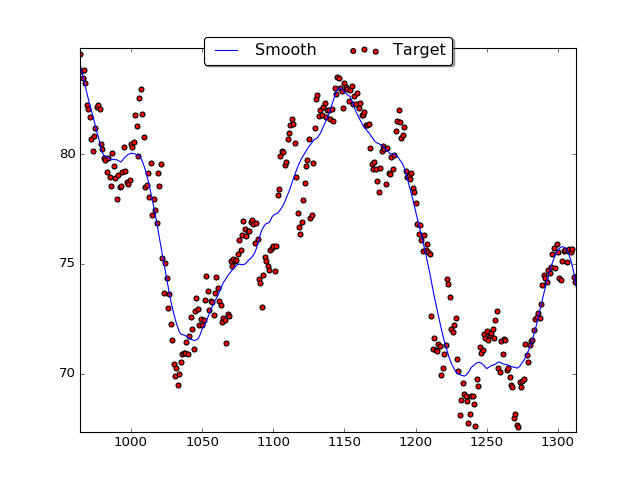
\includegraphics[width=0.8\textwidth]{figures/smooth.png}
\caption{\label{fig:data} Comparison between data points and the smooth plot}
\label{fig:smooth}
\end{figure}
\ \\


\subsection{Implementation}
\label{subsec:implementation}
Given all the features available: \textit{Open, Close, High, Low , Volume and Adjustment Close Price}, the firs step is to define which data will be used. The \textit{Adjustment Close Price} is the label
of this project, or, in other words, the data that this algorithm will try to predict. As studied in the Subsection \ref{subsec:Exploratory_visu}, all the remaining prices, except for the \textit{Volume},
are fully correlated. Therefore, \textit{Open, Close, High or Low} should perform as features well. However, any of this values are defined before the next business day starts. The consequence of it is that
the predictor would only work when, for example, the open price is given in the beginning of the day (as explained in \ref{subsec:data_exploration}, the open price is not always the same as the last close price).
Therefore, in order to perform this regression, the feature used will be the time. \\ 
\\
Once all the data to be used was defined, the next step is to split the data into train and test data. The method utilized for this project was the sklearn \textit{train\_test\_split}. This method
split arrays or matrices into random train and test subsets. The subset test was defined as 20\% of the whole data.\\
\\
Using the \textit{Support Vector Regressor}, the next step is to define the best regressor. The \textit{SVR} presents some tuning options, and in order to find the best option the method used
was the \textit{Pipeline} algorithm as defined in Subsection \ref{subsec:algorithm}. In order prevent excessing process, the first thing was to define the kernel, and The \textit{Radio Basis Function (RBF)}
kernel was the best fit. After it, all others parameters were left as variables to be defined in the process.\\


\subsection{Refinement}
\label{subsec:refinement}
In order to obtaing better results, studying the code was possible to find two options to improve it, in the pre-processing and in the learner. In the preprocessing, as explained in subsection \ref{subsec:preprocessing},
a filter was implemented to perform a smooth in the data. There are two options to tune this filter, the window that the algorithm will consider to perform the regression and the function's degree used in this 
regression. The metric used to evaluate how close was the new curve to the data, was used the $R² score$. So, in order to discover which pair of parameters would be better, it was simulated the learner with three
scores: The worst score, a mean score and the highest score. The results showed that the mean score was the right solution, therefore a pair of parameters that gave a score of 0.9942 was chosen.\\
\\
The other part of the algorithm needed to be improved was the learner. As explained in subsection \ref{subsec:implementation}, the \textit{Pipeline} method was implemented to obtain the best parameters
to the learner. Using the \textit{RBF} kernel, there was a couple of options to tune:
\begin{itemize}
 \item C: Penalty parameters\\
 \item Gamma: Kernel coefficient\\
\end{itemize}
\ \\
Once the \textit{Pipeline} process is implemented, the \textit{GridSearchVC} will be responsible to find the best set of parameters simulated, using the $R² score$ as value of decision.\\

\subsection{App development}
Before implementing any new method or algorithm, efforts were made to create an interface to visualize and interact with the process. In order to implement something simple
before moving to new high-end solutions, the solution was the framework python Web, with Javascript and HTML. The structure defined was: An algorithm in python responsible to launch the
Web server and perform the back end of the project, which is achieve data and perform the predictions. The HTML is rendered by the python to be visualized, and the javascript is responsible
to create the visual, graphics, interacting with the HTML and Python. The visualization was defined in three steps: Select the company and the period, select the algorithm to be used and the period
that will be predicted.\\
\\
To the visual part of this web solution was used \textit{jQWidgtes}, that can be downloaded on http://www.jqwidgets.com/, and \textit{Google Charts}, that can be downloaded on https://developers.google.com/chart/ .
These frameworks were defined after previous experience using them. And this solution was implemented to organize better the code and visualize each step of the process. As explained before, the
following three steps were defined:
\begin{itemize}
 \item Choosing Company: A list of available companies symbols is listed in order to be chosen. After choosing one, the Figure \ref{fig:nvs_stock_results} is displayed. The objective of this
 visualization is to understanding the stock prices over a period. This is just historical data, no preprocessing were made until this point. 
 \item Selecting Algorithm: A list of available algorithms is listed. After a choice is made, a graph is displayed presenting a comparison between the historical data and the result of the 
 prediction to all the data. In this step, when using the \textit{SVR} method, the pipeline algorithm will be used to find the best parameters. A box containing information about the regressor
 used and the \textbf{Test Score} will be showed. Illustrated on Figure \ref{fig:predict_svr}.
 \item Select Period to predict: A list of available days to predict will be displayed. It will have options from one day to forty five days. When the period is selected, a graph will be displayed
 showing the behavior of the stock prices over this period. Illustrated on Figure \ref{fig:predict_45days}.
\end{itemize}